%\part{Sem Confiança e Permissão}
\chapter{Prova de Trabalho}
\label{ch:capitulo3}

%Contanto que nosso livro-razão distribuído exija permissão para participar e possamos confiar que todas as partes sejam honestas, o sistema funcionará. Mas este tipo de design não pode ser escalado para ser usado por milhões de pessoas em todo o mundo.

%Os sistemas distribuídos feitos de participantes arbitrários são inerentemente não confiáveis. Algumas pessoas podem sair ocasionalmente. Isso significa que eles podem não saber das nossas transações quando as transmitimos. Outros podem estar ativamente tentando nos fraudar, dizendo que certas transações aconteceram ou não. Novas pessoas podem ingressar na rede e obter cópias conflitantes do livro-razão. Vamos dar uma olhada em como alguém pode tentar trapacear.%


%\newpage
%no meu livro esse paragrafo separa o inicio do capitulo 3 'prova de trabalho'

%\section**{O sistema de loteria que se auto executa}
%\paragraph{}

Este sistema de loteria, conforme projetado, tem dois problemas principais:

\begin{samepage}
\begin{enumerate}
\item Quem vai vender os bilhetes da loteria e escolher os números vencedores, se já determinamos que não podemos ter nenhum tipo de centralização que possa comprometer sua administração?
\item Como podemos garantir que o vencedor da loteria realmente registre boas transações no livro-razão, ao invés de tentar enganar o resto de nós?
\end{enumerate}
\end{samepage}

Se quisermos um sistema \textit{sem permissão} ao qual qualquer pessoa possa ingressar, temos que remover o requisito de confiança do sistema deixando-o totalmente \textit{sem necessidade de confiança}. Temos que criar um sistema que tenha as seguintes propriedades:


\begin{enumerate}
\item Deve ser possível para todos os integrantes gerar seus próprios bilhetes de loteria, uma vez que não podemos confiar em uma autoridade central;%removido a parte do powerball imagino q pq nao faz sentido em ptbr
\item Precisamos de alguma maneira para que haja custo ao gerar um bilhete, assim evitando que alguém possa monopolizar a loteria gerando um numero alto de bilhetes de graça. Como fazemos que uma possa precise gastar dinheiro para gerar um bilhete quando não há de quem comprar o bilhete? Faremos você comprar o bilhete do universo, queimando energia, um recurso custoso;
%Deve ser fácil para todos os outros participantes verificar se você ganhou na loteria apenas examinando seu bilhete, uma vez que não podemos confiar em ninguém para manter um registro da combinação vencedora;
\item Deve ser fácil para todos os outros participantes verificar se você ganhou na loteria apenas examinando seu bilhete, uma vez que não podemos confiar em ninguém para manter um registro da combinação vencedora, se ao invés disso, combinamos com antecedência uma faixa de valores se seu bilhete estiver dentro dessa faixa você ganha a loteria, usaremos uma ferramenta criptográfica chamada 'função Hash' para fazer isso;

%Precisamos de alguma forma de puni-lo se você ganhar na loteria, mas escrever transações inválidas no livro-razão, substituindo a confiança em pessoas específicas por confiança em incentivos e punições.
\end{enumerate}


%Na minha versao do livro nao tem essa explicação adicional sobre o powerball ela ta incluida na listagem acima.

Vamos falar de todos eles, um de cada vez. A explicação completa de como essa loteria funciona é provavelmente a coisa mais difícil de entender no Bitcoin, então vamos dedicar os próximos três capítulos para cobrir a solução em profundidade.

Sistemas de loteria centralizados padrão como Megasena são executados por alguém gerando um conjunto aleatório de números e um monte de bilhetes com números aleatórios neles. Normalmente, apenas um jogo possui os números que correspondem exatamente ao número aleatório secreto conhecido apenas pela organização que administra a Megasena. Uma vez que não podemos confiar na autoridade central, devemos permitir que qualquer um gere seus próprios números aleatórios.

Como iremos verificar o vencedor? Na Megasena, os proprietários da loteria conhecem a combinação vencedora. Já que não podemos ter isso em um sistema descentralizado, podemos então, criar um sistema onde todos possam concordar em uma faixa de números com antecedência, e se o seu número aleatório cair dentro da faixa, você ganha na loteria. Usaremos um truque criptográfico chamado função hash, para fazer isso. Vamos mergulhar em uma leve introdução a como usar o hash no próximo capítulo.

Finalmente, devemos encontrar uma maneira de puni-lo se você trapacear. Gerar números aleatórios, ou seja, bilhetes de loteria, é basicamente gratuito. Como fazemos para que você realmente tenha que gastar dinheiro para comprar bilhetes quando não há ninguém para vendê-los? Faremos você comprá-los do universo, gastando energia, um recurso escasso que não pode ser criado do nada. Isso será abordado no Capítulo 5.

\section*{Prova de trabalho: um quebra-cabeça assimétrico com uso intensivo de energia}
%\paragraph{}
A solução para esses três problemas é chamada de Prova de Trabalho. Na verdade, foi inventado muito antes do Bitcoin, mais precisamente, em 1993.

Precisamos tornar caro a “compra de bilhetes” para a loteria, caso contrário, as pessoas poderiam gerar um número ilimitado de bilhetes. O que é algo comprovadamente caro, mas isso não precisaria vir de nenhuma autoridade central?

Eu mencionei a física no início do livro, e é aqui que a física joga com o Bitcoin: a primeira lei da termodinâmica diz que a energia não pode ser criada nem destruída. Em outras palavras, não existe almoço grátis quando se trata de energia. A eletricidade é sempre cara porque é um recurso escasso que custa dinheiro real. Você tem que comprá-la dos produtores de energia ou operar sua própria usina. Em qualquer caso, você não pode obter algo do nada.

O conceito por trás da Prova de Trabalho é que você participa de um processo aleatório, semelhante a lançar um dado. Mas, em vez de um dado de seis lados, este tem tantos lados quanto a quantidade de átomos que existem no universo. Para lançar o dado e gerar números de loteria, seu computador deve realizar várias operações, que custam em termos de eletricidade.

Para ganhar na loteria, você deve produzir um número especial que é matematicamente derivado das transações que deseja gravar no livro-razão, mais um número aleatório (explicaremos os detalhes de como isso funciona no próximo capítulo).

Para encontrar esse número vencedor, você pode ter que rolar esse dado bilhões, trilhões ou quatrilhões de vezes, queimando centenas ou milhares de dólares em energia. Como o processo é baseado na aleatoriedade, é possível que todos gerem seus próprios bilhetes de loteria sem uma autoridade central, usando basicamente apenas um número aleatório que pode ser gerado por um software ou hardware e uma lista de transações que desejam gravar no livro-razão.

Agora, embora possa ter levado milhares de dólares para utilizar energia suficiente para encontrar o número aleatório correto, para que todos os outros na rede validem que você é um vencedor, eles precisam realizar algumas verificações básicas:

\begin{samepage}
\begin{enumerate}
\item O número que você forneceu é menor ou maior do que o limite mágico com o qual todos concordaram?
\item O número é de fato derivado matematicamente de um conjunto válido de transações que você deseja gravar no livro-razão?
\item As transações que vocês esta registrando são validas perante as regras do Bitcoin: sem gasto duplo, não gerando novos Bitcoin além do previsto e etc.
\end{enumerate}
\end{samepage}
%adicionado 
Prova de trabalho é um processo aleatório que requer muitas computações para achar o numero vencedor. Entretanto requer apenas uma única operação para verificar esta solução. Pense nele como palavras cruzadas ou sudoku. Pode demorar muito tempo para achar uma solução, mas dado as solução é de rápida verificação.
Isso torna o sistema de Prova de Trabalho \textit{assimétrico}: é muito difícil de gerar, mas muito fácil de ser validado.

Como você consumiu uma quantidade considerável de energia, e por sua vez, dinheiro jogando na loteria, deseja que todos aceitem o seu bilhete de loteria premiado. Portanto, você é incentivado a se comportar bem escrevendo apenas transações válidas no livro-razão.

Se você, por exemplo, tentar gastar um dinheiro que já foi gasto, então seu bilhete de loteria "vencedor" será rejeitado por todos os outros, e você perderá todo o dinheiro que gastou comprando a energia para criar o bilhete. Por outro lado, se você escrever transações válidas no livro-razão, iremos recompensá-lo em bitcoin para que você possa pagar suas contas de energia e ainda ter algum lucro.

O sistema de Prova de Trabalho tem a importante propriedade de ser \textit{caro no mundo real}. Assim, se você quisesse atacar a rede coagindo alguns de seus participantes, não só teria que vir à casa deles e assumir o hardware, mas também pagar suas contas de luz.

%Esse trecho nao vai agora na minha versao do livro.( na minha versao ele começa a falar sobre hashing e bits.)
%Hoje, estima-se que a rede Bitcoin como um todo gasta mais energia nesta loteria do que alguns países de médio porte. Essa é a quantidade de energia que você teria que usar para enganar a rede.

%Como os participantes provam que usaram essa energia? Discutiremos como a Prova de Trabalho é validada do ponto de vista matemático, à seguir.

%%%%%%%%%%%%%%%%%%%%%%%%%%%%%%%%%%%%%%%%%%%%%%%%%%%%%%%%%%%%%%%%%%%%%%%%%%%%%%%%%%%%%%%%%%%%%%%%%%%
Antes de podermos discutir como a Prova de Trabalho é validada, precisaremos de uma introdução rápida em Ciência da Computação sobre dois conceitos: bits e criação de hash.

\section*{Criando um Hash}
%\paragraph{}

O quebra-cabeça de Prova de Trabalho assimétrico do Bitcoin envolve o uso de uma função hash. Da álgebra básica, sabemos que uma função é uma caixa onde você \textit{insere} um valor de entrada \textit{x} e obtém um valor de saída \textit{f(x)}. Por exemplo, a função \textit{f(x)=2x} pega um valor e o multiplica por dois. Portanto, a entrada \textit{x=2} nos dá a \textit{saída f(x)=4}.

Uma função hash é uma função especial, onde você insere qualquer sequência de letras, números ou outros dados, como “Olá, mundo”, e obtém um número gigante que parece algo totalmente aleatório:

\begin{quote}{1111811713258219242661329357757490458455 \newline
4890446643616001126584346633541502095
}\end{quote}

A função hash particular usada acima na string "Hello, World" é chamada de sha256 e, por acaso, é a que o Bitcoin usa.

\begin{figure}
  \centering
  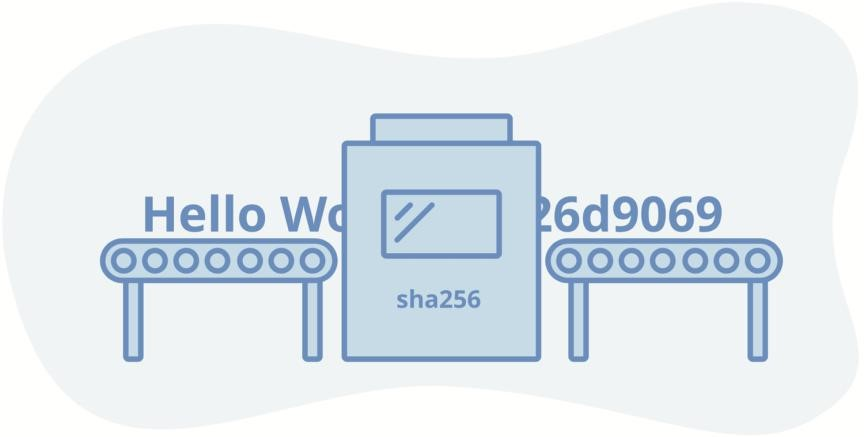
\includegraphics[width=7cm]{imagens/hash-capitulo-04.jpg}
  \caption*{\textit{\small Fazendo o hash de um string}}
\end{figure}

A função hash sha256 tem as seguintes propriedades que são úteis para nós:

\begin{enumerate}
\item A saída é determinística: você sempre obtém a mesma saída para a mesma entrada;
\item A saída é imprevisível: alterar apenas uma letra ou adicionar um espaço à string de entrada mudará drasticamente a saída, tanto que você não pode encontrar nenhuma correlação com os dados de entrada original;
\item É rápido calcular o hash para dados de entrada de qualquer tamanho;
\item É impossível encontrar duas strings que geram hash para a mesma saída;
\item Dado o hash de saída de sha256, é impossível retornar à string de entrada. Chamamos isso de função unilateral;
\item A saída é sempre um tamanho específico (256 bits para sha256).
\end{enumerate}

\section*{Uma introdução rápida sobre bits}
%\paragraph{}

O sistema numérico que você conhece e adora, composto dos números de 0 a 9, é chamado de \textit{decimal} porque possui dez dígitos. Os computadores, por outro lado, preferem um sistema numérico diferente, feito de uns e zeros, indicando a presença ou ausência de um sinal elétrico. Este sistema numérico é chamado de \textit{binário}.

No sistema decimal, você usa apenas os dígitos de 0 a 9. Se você usar apenas um dígito, poderá representar dez números diferentes, de 0 a 9. Se usar dois dígitos, poderá representar 10x10=100 números diferentes: 00, 01,\ldots a 99. Para três dígitos, você pode ter 10x10x10=1000 números: 000, 001,\ldots a 999.

Espero que você esteja começando a ver um padrão. Para descobrir o tamanho de um número que podemos representar com N dígitos, multiplicamos dez por ele mesmo N vezes. Em outras palavras, \(10^N\), ou 10 elevado à potência de N.

O binário funciona da mesma maneira. A única coisa que muda é o número de dígitos que estão disponíveis para nós. Embora estejamos acostumados com decimais com dez dígitos, um \textit{dígito binário} ou \textit{bit} só pode ter dois valores: zero e um.

Se 1 bit pode representar dois valores, então dois bits podem representar 4 valores: 00, 01, 10, 11. Você pode calcular isso multiplicando 2x2, pois cada dígito pode ter dois valores.

Três bits podem representar 2 x 2 x 2 = \(2^3\) = 8 valores, que são 000, 001, 010, 011, 100, 101, 110, 111.

Portanto, um número \textit{binário} de N \textit{bits} pode ser representado como \(2^N\) valores diferentes.

Portanto, o número de valores exclusivos que você pode representar com 256 bits, o tamanho da função de hashing sha256, é \(2^{256}\). Esse é um número gigante, quase inconcebível para a mente humana. Representado em decimal, esse número tem 78 dígitos. Para colocar isso em perspectiva, isso é mais ou menos o número estimado de átomos em todo o universo conhecido.


\begin{multline}
\begin{aligned}
2^{256} = & 115.792.089.237.316.195.423.570.985.008.\\
& 687.907.853.269.984.665.640.564.039.457.\\
& 584.007.913.129.639.936
\end{aligned}
\end{multline}


Este é o número de saídas possíveis quando você faz o hash de qualquer string com a função de hash sha256. Portanto, é efetivamente impossível prever como será o número produzido por essa função. Seria como prever 256 jogadas de moeda em sequência ou adivinhar a localização de um átomo específico que escolhi em algum lugar do universo.

Este número é muito longo para continuar escrevendo, então diremos apenas \(2^{256}\) de agora em diante, mas espero que isso acione uma imagem mental de um universo de possibilidades para você.

\section*{Vamos transformar algumas strings em hash}
%\paragraph{}

Aqui estão algumas strings de exemplo e seus hashes sha256. O resultado está em números decimais, embora dentro de um computador eles apareceriam como uma sequência binária de uns e zeros.

O objetivo aqui é demonstrar como o número muda drasticamente com base em uma pequena mudança na string de entrada. Você não pode prever a saída produzida pela função hash com base no que você colocou nela:


\begin{quote}{"Hello World!"\newline
52740724284578854442640185928423074974\newline
81806529570658746454048816174655413720\newline
}\end{quote}


\begin{samepage}
\begin{quote}{"Hello World!!"\newline
958633198749395357316023441946434972583\newline
74513872780665335270495834770720452323\newline
}\end{quote}
\end{samepage}

Não há como ninguém, nem mesmo um computador, olhar para o número de aparência aleatória resultante e descobrir a string que o criou. Se você quiser brincar com o sha256, há alguns sites online onde você pode experimentar fazer o hash de qualquer informação que desejar. por exemplo \url{https://passwordsgenerator.net/sha256-hash-generator/}

\section*{Criando um hash para ganhar na loteria de prova de trabalho}
%\paragraph{}
 
Tudo bem, agora estamos prontos para falar sobre a parte chave da magia. Dissemos que há \(2^{256}\) valores de saída de sha256 possíveis no total. Para tornar mais fácil de entender, vamos fingir que há apenas um total de 1000 saídas hash possíveis.

O nosso sistema de loteria funciona assim:

\begin{enumerate}
\item Ana anuncia que deseja enviar R\$2,00 para Bruno;
\item Todo mundo que quer tentar a sorte na loteria pega esta transação “Ana envia R\$2,00 para Bruno”, adicionando um número aleatório chamado \textit{nonce} (número usado apenas uma vez) no final. Isso é para ter certeza de que a string que eles estão fazendo o hash é diferente de qualquer outra pessoa, ajudando-os a encontrar um número vencedor na loteria;
\item Se esse número for menor do que o \textit{Número Alvo} (veremos isso em um segundo), eles ganham na loteria;
\item Se o número que eles obtiverem for maior do que o número alvo, eles tentam fazer o hash novamente, adicionando nonces aleatórios: “Ana envia R\$2,00 para Bruno com nonce = 12345”, “Ana envia R\$2,00 para Bruno com nonce = 92435”, “Ana envia R\$2,00 para Bruno nonce = 132849012348092134” e assim por diante, até que o número hash resultante seja menor que o \textit{Número Alvo}.
\end{enumerate}

Pode levar muitas, muitas tentativas para encontrar um hash que seja menor que o número alvo. Portanto, a ideia aqui é esta: se houver 1000 hashes possíveis e definirmos o número alvo como 100, qual porcentagem de hashes está abaixo do alvo?

Esta é a matemática básica: de 1000 números possíveis, de zero a 999, existem 100 números que são menores que 100 e 900 números que são maiores. Portanto, 100/1000 ou 10\% dos hashes são menores que o destino. Então, se você fizer um hash com qualquer string e sua função hash produzir 1000 saídas diferentes, você espera obter um hash abaixo do alvo limitado a 100, cerca de 10\% do tempo.

É assim que a loteria funciona: nós definimos um \textit{alvo} e todos concordamos com ele (falaremos sobre como isso funciona em breve). Então, pegamos as transações sobre as quais as pessoas estão nos contando e fazemos o hash, adicionando um nonce aleatório no final. Assim que alguém encontra um hash que está dentro do limite imposto pelo alvo, nós o anunciamos para todos na rede:

Olá pessoal:
\begin{itemize}
\item Peguei as transações: "Ana envia R\$2,00 para Bruno, Carol envia R\$5,00 para Ana";
\item Adicionei o nonce "32895";
\item O resultado foi um hash com retorno 42, que é menor que o alvo limite de 100;
\item Aqui está minha prova de trabalho: os dados da transação, o nonce que usei e o hash que foi produzido com base nessas entradas.
\end{itemize}

Para isso, talvez seja necessário bilhões de tentativas de hash para conseguir o resultado, gastando milhares de dólares em energia, mas todos podem imediatamente validar que fiz certo porque eles podem fazer o hash em uma única tentativa, já que dei a entrada e o saída esperada. Lembre-se de que os hashes são impossíveis de serem revertidos, mas são fáceis de serem calculados!

Como isso está ligado ao gasto de energia? Bem, já dissemos que o conjunto de todos os hashes possíveis é na verdade um número gigante que é quase tão grande quanto o número de átomos no universo. Agora podemos definir o \textit{alvo} como baixo para que apenas uma pequena fração dos hashes sejam válidos. Isso significa que qualquer pessoa que quiser encontrar um hash válido terá que gastar uma grande quantidade de tempo e processamento o que significa que terá que gastar eletricidade, para encontrar um número de hash menor que nosso alvo.

Quanto menor o alvo, mais tentativas serão necessárias para encontrar um número que funcione. Quanto maior o alvo, mais rápido podemos encontrar um hash vencedor.